\documentclass[10pt,a4paper]{article}

\usepackage[utf8x]{inputenc}
\usepackage{ucs}
\usepackage[francais]{babel}
\usepackage[T1]{fontenc}

\usepackage{amsmath}
\usepackage{amsfonts}
\usepackage{amssymb}

\usepackage{multirow}
\usepackage{graphicx}

\usepackage{boxedminipage}
\addtolength{\fboxsep}{3pt}

\title{Cahier des charges de Bob-Project (TD 33)}
\author{LAFON Sylvain, LEVASSEUR Thomas et MAINGRET François}

\begin{document}
	\maketitle
	\tableofcontents
	\newpage
	\part{Introduction}
		Le bricolage et le jardinage etants à la mode des derniers temps, le site Brico-Bob vise à proposer à des utilisateurs de profils variés, aussi bien
la ménagère que le retraité ou que les jeunes couples, du matériel à la vente ou à la location.
Ce site étant de nature commerciale, il se doit d'etre visuellement attractif et d'etre ergonomique. La présentation des produits devra etre simple, claire, et 
bien organisée, l'utilisateur devra pouvoir trouver un produit le plus rapidement possible afin qu'il ne se lasse pas du site et qu'il achète le plus de prosuits
possible ( De plus, il existera une fonction pour rechercher un produit selon differents critères. De la publicité sur certaines pages du site pourra influencer
le client.
Chaque utilisateur du site devra s'inscrire en fournissant un login et un mot de passe pour  faire ses achats, ses informations personnelles ( nom, adresse... )
ne seront demandées que lors de la validation de la commande ). Chaque membre du site pourra poster des avis, et noter les differents produits, ainsi que poser
des questions techniques.
Enfin, l'administrateur du site pourra gerer simplement, depuis une fenetre speciale, le contenu du magasin, et les membres.

	\newpage
	\part{Fonctionnalités}
		\section{Cas d'utilisation}
			\subsection{Description des acteurs}
				Il existe 3 acteurs principaux au sein de cette application :

\subsubsection{internaute} 

l'internaute est un visiteur de passage, qui peut venir pour la premiere fois sur le site, pour rechercher et consulter des produits, par exemple pour comparer
les prix avec la concurence. il peut également etre un visiteur regulier qui verifie les promotions en cours. bien que cet internaute puisse accèder a une grande partie des pages du site, ses possibilités sont limités, il a donc la posibilité de s'inscrire afin de devenir membre

\subsubsection{membre}

le membre est un internaute qui s'est inscrit au site, en ne donnant aucune information personnelle, apart son e-mail, necessaire en cas de problème. 
il aura la possibilité de poser des questions sur des produits, de donner son avis ainsi que de noter les articles, mais surtout d'acheter ou de louer des produits.
Le membre ne fournirra ses coordonnées que lors de sa premiere commande, ce pour lui demander les informations necessaires en temps voulu, qu'il ne fournisse pas son nom alors que ce n'est pas encore nesessaire, pour des questions de protection de la vie privée.

\subsubsection{admin}

les administrateurs du site pourront faire tout ce que les membres peuvent faire, mais auront accès a un panneau d'administration, que nous verrons en details plus tard dans ce dossier, qui leur permettra de gerer tout le contenu du site ainsi que les membres, sans passer directement pas le SGBD, ce qui est plus simple d'utilisation (un admin pourra ajouter des produits, promotions, bannir un membre... voir user case  ).
Toutefois, l'administateur ne pourra pas modifier un message ecrit pas un membre, ni les informations sur un membre.

			\subsection{Description des cas d'utilisation}
				\begin{description}
	\item[S'inscrire : ]	
		Permet a un internaute de devenir membre du site en entrant un pseudonyme et un mot de passe.
	\item[Consulter Catégories : ]	
		Permet à l'utilisateur de parcourir la liste des catégories afin de faire une recherche "manuelle" d'un produit
	\item[Consulter Fiche Produit : ]
		L'utilisateur consulte les informations relatives à un produit.
	\item[Se Connecter : ]
		L'internaute déja inscrit entre son login et son mot de passe afin de de conecter en tant que membre ( ou admin )
	\item[Se Déconnecter : ]	
		L'internaute déja conecté se déconnecte et perds son statut de membre ( ou d'admin )	
	\item[Evaluer un Produit : ]
		L'internaute déja connecté donne une note et un commentaire sur un produit. Il peut également poser une question sur un produit.
	\item[Mettre à jour ses infos : ]
		L'internaute déja connecté met a jour les informations qu'il a fournies au sites.
	\item[Ajouter un produit : ]
		L'admin ajoute un produit dans la base de donnée en passant par le panneau admin.	
	\item[Ajouter une catégorie : ]	
		L'admin ajoute une catégorie dans la base de donnée en passant par le panneau admin.	
	\item[Supprimer un produit : ]	
		L'admin supprume un produit de la base de donnée en passant par le panneau admin.
	\item[Supprimer une catégorie : ]
		L'admin supprime une catégorie de la base de donnée en passant par le panneau admin.
	\item[Supprimer une évaluation : ]	
		L'admin supprime l'évaluation d'un produit ( par exemple en cas de commentaire injurieux, de publicité ou de spam )	
	\item[Bannir membre : ]	
		L'admin supprime un membre de la base de donnée si celui-ci utilise mal le site ( spam de commentaires d'un produit )
\end{description}

			\subsection{Description synthétique}
				\subsubsection{Inscription, connexion et deconnexion}
					1 Le système propose à l'internaute de s'inscrire.
2 L'internaute clique sur "s'inscrire".
3 Le système demande à l'internaute de lui fournir un nom de compte, un mot de passe et une vérification du mot de passe.
4 L'internet entre les informations demandées.
5 L'internaute clique sur "s'inscrire".
6 L'internaute est inscrit et connecter.

Exceptions: 
			5a L'internaute a entrer un pseudo éxistant.
			6 Le systeme affiche "Pseudo déja utiliser".
			7 Le système propose de nouveau à l'internaute de s'incrire.
			
			5a L'internaute a entrer deux mot de passe differents.
			6 Le système affiche "Les mots de passe ne sont pas identiques".
			7 Le système propose de rentrer à nouveau les mots de passe.

\begin{boxedminipage}[t]{12cm}
	\begin{itemize}
		\item Système : Site web "Chez Bob"
		\item Acteur : Internaute
		\item Objectif : Inscrire un compte
		\item Pré-condition : (aucune)
	\end{itemize}

	\renewcommand\theenumi{\arabic{enumi}}
	\renewcommand\labelenumi{\theenumi .}
	\renewcommand\theenumii{\Alph{enumii}}
	\renewcommand\labelenumii{(\theenumii)}
	\paragraph{Scénario :} 
	\begin{enumerate}
		\item \label{sc1l1} un item
	\end{enumerate}
\end{boxedminipage}
\newpage

\begin{boxedminipage}[t]{12cm}
	\begin{itemize}
		\item Système : Site web "Chez Bob"
		\item Acteur : Internaute
		\item Objectif : Se connecter sur le compte de l'utilisateur
		\item Pré-condition : L'utilisateur est enregistré
	\end{itemize}

	\renewcommand\theenumi{\arabic{enumi}}
	\renewcommand\labelenumi{\theenumi .}
	\renewcommand\theenumii{\Alph{enumii}}
	\renewcommand\labelenumii{(\theenumii)}
	\paragraph{Scénario : }
	\begin{enumerate}
		\item \label{sc2l1} Le système propose à l'utilisateur de se connecter à son compte.
		\item \label{sc2l2} L'utilisateur clique sur "se connecter".
		\item \label{sc2l3} Le système demande le nom de compte et le mot de passe de l'utilisateur.
		\item \label{sc2l4} L'internaute entre les informations demandées.
		\item \label{sc2l5} L'internaute clique sur "se connecter".
		\item \label{sc2l6} L'internaute est connecté à son compte.
	\end{enumerate}

	\renewcommand\theenumi{\Alph{enumi}}
	\renewcommand\labelenumi{\theenumi )}
	\renewcommand\theenumii{\arabic{enumii}}
	\renewcommand\labelenumii{\theenumii .}
	\paragraph{Exceptions :} 
	\begin{enumerate}
		\item
		\begin{enumerate}
			\addtocounter{enumii}{4}
			\item Une des informations ou les deux demandées ne correspondent pas.
			\item Le système affiche un message d'erreur
			\item Retour à \ref{sc2l3}
		\end{enumerate}
	\end{enumerate}
\end{boxedminipage}
\newline

\begin{boxedminipage}[t]{12cm}
	\begin{itemize}
		\item Système : Site web "Chez Bob"
		\item Acteur : Internaute
		\item Objectif : Se déconnecter de son compte
		\item Pré-condition : L'utilisateur est connecté à son compte
	\end{itemize}

	\renewcommand\theenumi{\arabic{enumi}}
	\renewcommand\labelenumi{\theenumi .}
	\renewcommand\theenumii{\Alph{enumii}}
	\renewcommand\labelenumii{(\theenumii)}
	\paragraph{Scénario :} 
	\begin{enumerate}
		\item \label{sc3l1} Le système propose à l'utilisateur de se déconnecter de son compte.
		\item \label{sc3l2} L'utilisateur clique sur "se déconnecter".
		\item \label{sc3l3} Le système déconnecte le membre de son compte.
		\item \label{sc3l4} Le système redirige l'internaute vers l'accueil.
	\end{enumerate}
\end{boxedminipage}
\newpage

% On remet les valeurs qui sont là par défaut.
\renewcommand\theenumi{\arabic{enumi}}
\renewcommand\labelenumi{\theenumi .}
\renewcommand\theenumii{\Alph{enumii}}
\renewcommand\labelenumii{(\theenumii)}
				\subsubsection{Recherche d'un produit}
					%
%  Contient les 3 scénarios pour la recherche
%
\begin{boxedminipage}[t]{12cm}
	\begin{itemize}
		\item Système : Bob-Project
		\item Acteur primaire : internaute
		\item Objectif : Rechercher un produit (via la barre)
		\item Préconditions : (aucune)
	\end{itemize}

	\renewcommand\theenumi{\arabic{enumi}}
	\renewcommand\labelenumi{\theenumi .}
	\renewcommand\theenumii{\Alph{enumii}}
	\renewcommand\labelenumii{(\theenumii)}
	\paragraph*{Scénario 1 :}
	\begin{enumerate}
		\item \label{sr1l1} L'utilisateur entre un nom de produit à rechercher
		\item \label{sr1l2} Le système recherche tout d'abord le nom exact
		\item \label{sr1l3} Le système recherche ensuite les noms qui ressemblent
		\item \label{sr1l4} Le système affiche une page de résultat dans laquelle on trouve les différents produits.
	\end{enumerate}


	\renewcommand\theenumi{\Alph{enumi}}
	\renewcommand\labelenumi{\theenumi )}
	\renewcommand\theenumii{\arabic{enumii}}
	\renewcommand\labelenumii{\theenumii .}
	\paragraph*{Exceptions :}
	\begin{enumerate}
		\item
			\begin{enumerate}
				\item L'utilisateur valide en ayant laissé un champ vide
				\item Le système renvoie l'utilisateur vers la page de Recherche avancée en lui disant que le champ n'était pas rempli
			\end{enumerate}
		\item
			\begin{enumerate}
				\addtocounter{enumii}{1}
				\item Le système ne trouve aucun résultat
				\item Le système recherche ensuite les noms qui ressemblent
				\item Le système affiche une page de résultat dans laquelle on trouve les produits avec un nom ressemblant, et propose une correction de la recherche.
			\end{enumerate} 
		\item
			\begin{enumerate}
				\addtocounter{enumii}{2}
				\item Le système ne trouve aucun résultat
				\item Le système renvoie l'utilisateur vers la page de Recherche avancée en lui disant que rien n'à pu être trouvé
			\end{enumerate}
		\item
			\begin{enumerate}
				\addtocounter{enumii}{1}
				\item Le système trouve beaucoup de résultats
				\item Le système affiche une page de résultat dans laquelle on trouve les différents produits avec un message comme quoi une recherche avancée pourrait affiner le résultat.
			\end{enumerate}	
	\end{enumerate}
\end{boxedminipage}
\newpage
\begin{boxedminipage}[t]{12cm}
	\begin{itemize}
		\item Système : Bob-Project
		\item Acteur primaire : internaute
		\item Objectif : Rechercher un produit (via la page de Recherche avancée)
		\item Préconditions : être en train d'aller sur la page (redirection ou lien)
	\end{itemize}

	\renewcommand\theenumi{\arabic{enumi}}
	\renewcommand\labelenumi{\theenumi .}
	\renewcommand\theenumii{\Alph{enumii}}
	\renewcommand\labelenumii{(\theenumii)}
	\paragraph*{Scénario 2 :}
	\begin{enumerate}
		\item \label{sr2l1} Le système présente un grand formulaire contenant notemment :
			\begin{itemize}
				\item Nom du produit (*)
				\item Catégorie du produit
				\item Prix du produit
				\item (autres critères comme la marque)
			\end{itemize}
		\item \label{sr2l2} Le système lance la recherche avec la recherche exacte
		\item \label{sr2l3} Le système lance la recherche sur le nom
		\item \label{sr2l4} Le système lance la recherche sur les produits qui ont des points communs
		\item \label{sr2l5} Le système affiche une page de résultat avec le resultat du \ref{sr2l2} visible et demande si les autres résultats peuvent être affichés
	\end{enumerate}

	\renewcommand\theenumi{\Alph{enumi}}
	\renewcommand\labelenumi{\theenumi )}
	\renewcommand\theenumii{\arabic{enumii}}
	\renewcommand\labelenumii{\theenumii .}
	\paragraph*{Exceptions :}
	\begin{enumerate}
		\item
			\begin{enumerate}
				\item L'utilisateur ne rentre pas le nom du produit (obligatoire)
				\item Le système affiche un message d'erreur
				\item Retour à \ref{sr2l1}
			\end{enumerate}
		\item
			\begin{enumerate}
				\addtocounter{enumii}{3}
				\item Vraiment aucun résultat
				\item Le système envoie un message d'excuse : aucun produit n'a pu être trouvé
				\item Retour à \ref{sr2l1}
			\end{enumerate}
	\end{enumerate}
\end{boxedminipage}
\newpage
\begin{boxedminipage}[t]{12cm}
	\begin{itemize}
		\item Système : Bob-Project
		\item Acteur primaire : internaute
		\item Objectif : Rechercher un produit (via l'exploration)
		\item Préconditions : (aucune)
	\end{itemize}

	\renewcommand\theenumi{\arabic{enumi}}
	\renewcommand\labelenumi{\theenumi .}
	\renewcommand\theenumii{\Alph{enumii}}
	\renewcommand\labelenumii{(\theenumii)}
	\paragraph*{Scénario 3 :}
	\begin{enumerate}
		\item \label{sr3l1} L'utilisateur passe la souris sur Acheter ou Louer (menu)
		\item \label{sr3l2} L'utilisateur clique sur une catégorie
		\item \label{sr3l3} Le système affiche la page de la sous-catégorie
		\item \label{sr3l4} L'utilisateur clique sur un produit
		\item \label{sr3l5} (L'utilisateur à trouvé son produit)
	\end{enumerate}

	\renewcommand\theenumi{\Alph{enumi}}
	\renewcommand\labelenumi{\theenumi )}
	\renewcommand\theenumii{\arabic{enumii}}
	\renewcommand\labelenumii{\theenumii .}
	\paragraph*{Exceptions :}
	\begin{enumerate}
		\item
			\begin{enumerate}
				\item L'utilisateur clique sur Acheter ou Louer
				\item Le système affiche la page des catégories
				\item Retour à \ref{sr3l2}
			\end{enumerate}
		\item
			\begin{enumerate}
				\addtocounter{enumii}{3}
				\item L'utilisateur clique sur une autre sous-catégorie
				\item Retour à \ref{sr3l3}
			\end{enumerate}
		\item
			\begin{enumerate}
				\addtocounter{enumii}{4}
				\item (L'utilisateur ne trouve pas son produit)
				\item Rien ne se passe : il peut continuer à explorer ou bien passer à autre chose ou encore utiliser la barre de recherche
			\end{enumerate}
	\end{enumerate}
\end{boxedminipage}
\newpage

\renewcommand\theenumi{\arabic{enumi}}
\renewcommand\labelenumi{\theenumi .}
\renewcommand\theenumii{\Alph{enumii}}
\renewcommand\labelenumii{(\theenumii)}
				\subsubsection{Affichage d'un produit}
					\begin{boxedminipage}[t]{12cm}
  \begin{itemize}
		\item Système : Site web "Chez Bob"
		\item Acteur : Internaute
		\item Objectif : Visualiser Fiche Produit
		\item Pré-condition : L'utilisateur à trouvé un produit ou une liste de produits
	\end{itemize}

	\paragraph{Scénario : }
	\begin{enumerate}
		\item \label{sll1} Le système propose à l'utilisateur un ou plusieurs produits a visualiser.
		\item \label{sll2} L'utilisateur sélectionne le produit qu'il souhaite visualiser
		\item \label{sll3} Le système recherche les info relatives au produit dans la DB
		\item \label{sll4} Le système affiche les informations relatives au produit ( Nom, prix, description, photo, note, commentaires... )
	\end{enumerate}

\newline
			\subsection{Diagramme de cas d'utilisation}
				Le diagramme de cas d'utilisation est fourni en annexe
				\newline
					
				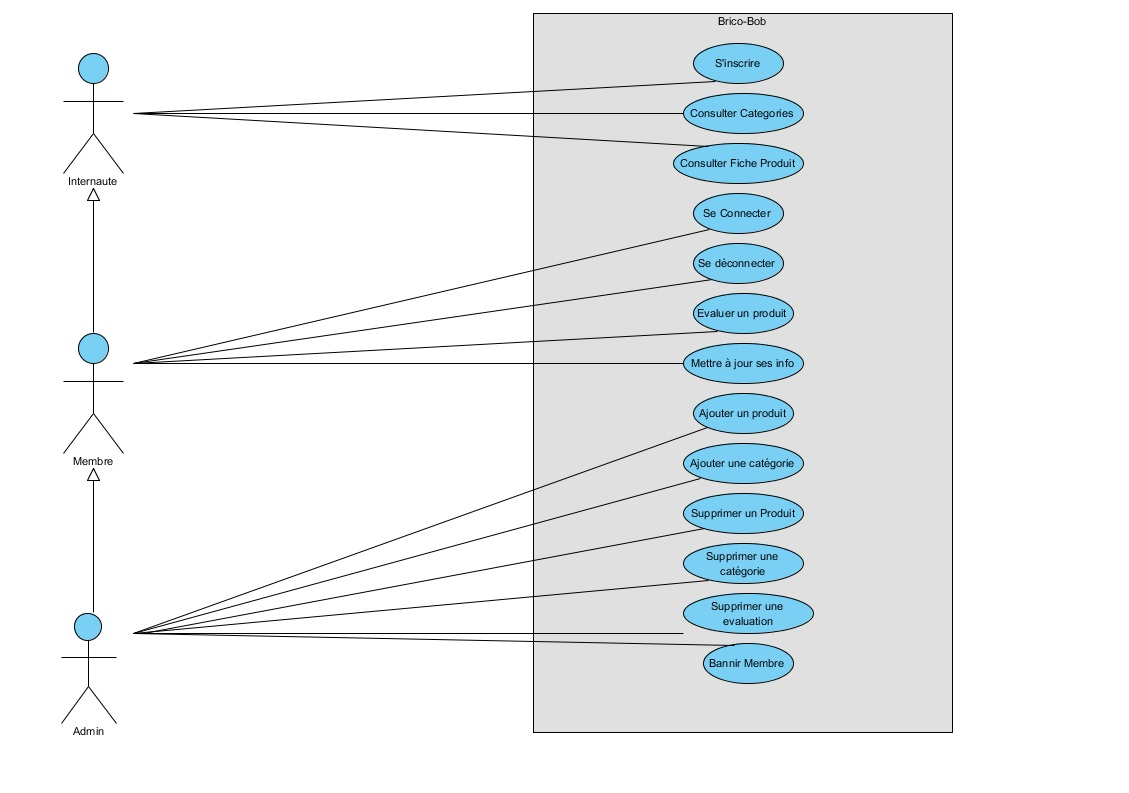
\includegraphics[scale=0.5]{cas/diagramme.jpg}
			\subsection{Contraintes non fonctionnelles}
				\paragraph{Confidentialité}

Lors de l'inscription, l'internaute n'entre pas ses données personnelles ( Nom, Adresse ... ) afin de ne pas lui demander trop vite
d'informations personelles, ce qui pourrait être perçu comme une intrusion dans sa vie privée alors que ces données ne sont pas encore
nécessaires. Elle lui seront demandées seulement lors de la validation d'une commande ( Utilisation non prévue dans le cadre de cette étude )

\paragraph{Rapidité de Réponse}
	
La grande majorité des images du site seront enregistrées dans un format tel qu'elles seront légères et rapides a charger pour l'internaute.
Le code javascript et les "animations" seront réduites au stricte minimum afin de ne pas ralentir le site.

\paragraph{Charte graphique}

(En annexe)

\paragraph{Normes Ergonomiques}
	
(En annexe)

\paragraph{Portabilité de l'application}
	
Cette application sera conçue de sorte qu'elle soit accessible depuis n'importe quel navigateur récent. Certains éléments graphiques différèrent légèrement selon le navigateur de l'utilisateur ( par exemple une très légère différence sur les couleurs du fond, du a une non-compatibilité de certaines propriétés CSS3 par certains navigateurs) mais cela n'altèrera en rien les fonctionnalités et le confort de navigation.
La résolution d'écran nécessaire au bon affichage du site sera assez faible pour que le plus grand nombre puisse l'utiliser.

\paragraph{Modification du contexte}
	
Le site Brico-Bob sera conçu de telle sorte que ce modèle de magasin en ligne sera transposable à d'autres secteurs ( par exemple de la vente de chocolats ou  une agence de voyages... ) Il suffira de modifier le contenu de la base de données pour répondre a de nouveaux besoins.

\paragraph{Matériel et logiciels utilisés}
	
Le code a été écrit intégralement sur Notepad ++, qui est simple d'utilisation et très clair.
Les tests ont été utilisés grâce à WAMP et nous avons utilisés mysql pour le stockage des données.
Nous avons utilisés GitHub afin de synchroniser notre travail et de nous organiser.
Des tests ont été effectués sur Internet Explorer 7,8,9 Google Chrome et Mozilla Firefox

	\newpage			
	\part{Données}
		\section{Dictionnaire de données}
			\documentclass{report}

\usepackage[latin1]{inputenc}
\usepackage[T1]{fontenc}
\usepackage[francais]{babel}

\begin{document}
\begin{tabular}{|c|c|c|}

\hline
\begin{bf}Noms\end{bf} & \begin{bf} Type \end{bf} & \begin{bf} Commentaires non evidents\end{bf}\\
\hline
numIndividu & Entier & Nom de l'individu.\\
\hline
nomIndividu & Chaine de caracteres & \\
\hline
prenomIndividu & Chaine de caracteres & \\
\hline
adresseIndividu & Chaine de caracteres & \\
\hline
telephoneIndividu & Entier & \\
\hline
idAdmin & Entier & \\
\hline
idUtilisateur & Entier & \\
\hline
pseudoUtilisateur & Chaine & \\
\hline
passUtilisateur & Chaine & \\
\hline
mailUtilisateur & Chaine & \\
\hline
idRep & Entier & \\
\hline
idAdmin & Entier & \\
\hline
reponse & Chaine & \\
\hline
dateRep & Date & \\
\hline
idEval & Entier & \\
\hline
idReponse & Entier & \\
\hline
idEval & Entier & \\
\hline
dateEval & Date & \\
\hline
noteEval & Entier & \\
\hline
commentaireEval & Texte & \\
\hline
idUtilisateur & Entier & \\
\hline
idProduit & Entier & \\
\hline
idEval & Entier & \\
\hline
idImage & Entier & \\
\hline
image & BLOB & \\
\hline
titre & Chaine & \\
\hline
legende & Chaine & \\
\hline
idCible & Entier & \\
\hline
idCat & Entier & \\
\hline
descriptionCat & Chaine & \\
\hline
nomCat & Chaine & \\
\hline
idParent & Entier & \\
\hline
idProd & Entier & \\
\hline
nomProd & Entier & \\
\hline
libelle & Chaine de caracteres & \\
\hline
imageProd & BLOB & \\
\hline
stockProd & Entier & \\
\hline
nbVentesProd & Entier & \\
\hline
nbLocProd & Entier & \\
\hline
prixProdVente & Entier & \\
\hline
prixProdLoc & Entier & \\
\hline
idCatProd & Entier & \\
\hline
idPub & Entier & \\
\hline
idCible & Entier & \\
\hline
offrePub & Chaine & \\
\hline
imgPub & BLOB & Image de la pub.\\
\hline

\end{tabular}

\end{document}
		\section{Structures de données}
			\subsection{Schéma relationnel}
				Le schéma relationnel est fourni en annexe
				\newline
					
				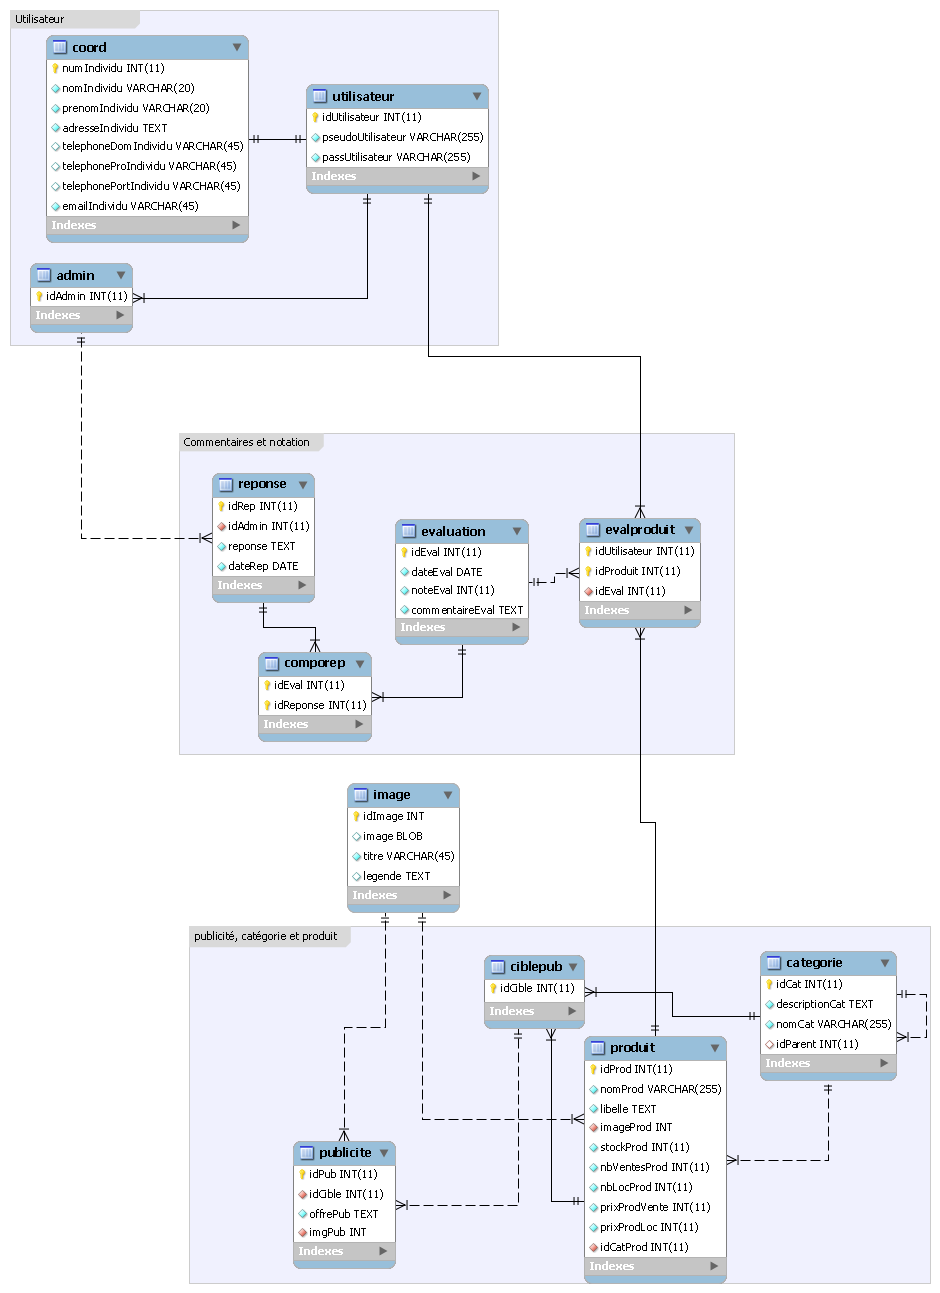
\includegraphics[scale=0.2]{donnees/SR.png}
			\subsection{Objets}
				\subsubsection{Diagramme de classe}
					Le diagramme de classe est fourni en annexe
					\newline
					
					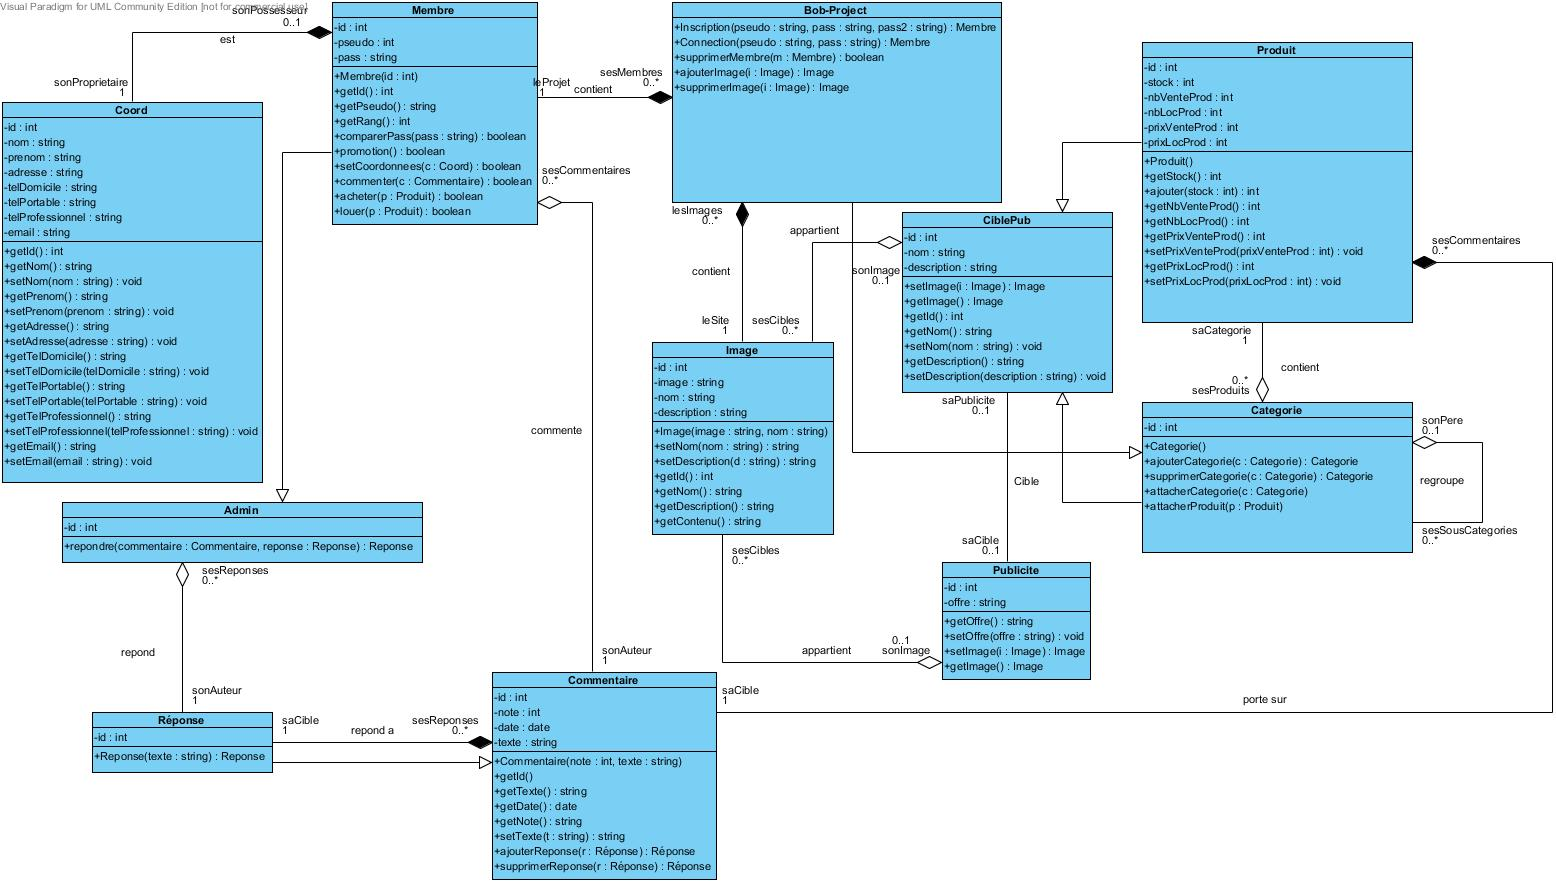
\includegraphics[scale=0.2]{donnees/classes.jpg}
				\subsubsection{Justification des cardinalités}
					\paragraph{Classe Membre :} Peut représenter toute personne enregistrée sur le site.\\

\begin{tabular}{|c|c|c|c|c|}
	\hline
		\multirow{2}*{\begin{bf}Classe\end{bf}} &
		\multirow{2}*{\begin{bf}Nom\end{bf}} &
		\multicolumn{3}{c|}{\begin{bf}Cardinalité\end{bf}} \\
	\cline{3-5}
		 & & \begin{bf}nom\end{bf} & \begin{bf}de\end{bf} & \begin{bf}à\end{bf} \\
	\hline
	\hline
		Coord & est & sonPossesseur & 0 & 1 \\
	\hline
		\multicolumn{5}{|c|}{Au départ, on ne va pas demander les informations du membre,} \\
		\multicolumn{5}{|c|}{on attendra les premiers achats (/locations) pour cela.} \\
	\hline
	\hline
		Commentaire & commente & sesCommentaires & 0 & * \\
	\hline
		\multicolumn{5}{|c|}{On poste autant de commentaires que l'on veut} \\
	\hline
\end{tabular}

\paragraph{Classe Categorie :} Permet de ranger les produits\\

\begin{tabular}{|c|c|c|c|c|}
	\hline
		\multirow{2}*{\begin{bf}Classe\end{bf}} &
		\multirow{2}*{\begin{bf}Nom\end{bf}} &
		\multicolumn{3}{c|}{\begin{bf}Cardinalité\end{bf}} \\
	\cline{3-5}
		 & & \begin{bf}nom\end{bf} & \begin{bf}de\end{bf} & \begin{bf}à\end{bf} \\
	\hline
	\hline
		\multirow{2}*{Categorie} & \multirow{2}*{regroupe} & sesSousCategories & 0 & * \\
	\cline{3-5}
		 & & sonPere & 0 & 1 \\
	\hline
		\multicolumn{5}{|c|}{Toute categorie peut avoir autant de sous-categorie qu'elle veut} \\
		\multicolumn{5}{|c|}{Bob-Project est la seule categorie qui n'a aucun pere} \\
		\multicolumn{5}{|c|}{Les autres n'en ont qu'un.} \\
	\hline
	\hline
		Commentaire & commente & sesCommentaires & 0 & * \\
	\hline
		\multicolumn{5}{|c|}{On poste autant de commentaires que l'on veut} \\
	\hline
\end{tabular}
				\subsubsection{Historique}
					Les classes d'informations personnelles, si non mises à jour, ne peuvent rester plus de 3 ans (loi) ainsi, contrairement à la classe Membre, la classe Coord à une durée de vie\\

Les classes de commentaires sont également soumises à une certaine durée de vie (mettons un an, par exemple)
				\subsubsection{Contraintes non modélisables}
					\paragraph{Forme des adresses mail}

Les e-mails doivent être de la forme [Chaine de caractères]@[chaine de caractères].[Chaine de caractères,4 caractères au maximum (.fr,.com...)]

\paragraph{Taille et forme des mots de passe}

Les mots de passe doivent avoir une taille comprise entre 4 et 255 caractères. Il faut que la casse soit respectée et que l'on puisse mettre des caractères spéciaux et numériques.

\paragraph{Numéro de téléphone}

Les numéros de téléphone sont stockés dans une variables String mais ne doivent contenir que des chiffres.

\paragraph{Chaines de caractères}

Les chaines de caractères ne peuvent contenir des espaces.

\paragraph{Cryptage des mots de passe}

Les mots de passe sont crypter (sha1) avant d'être stocker dans la base de données pour ne pas être lisible au premier coup d'œil dans la base de données.
	\newpage
	\part{Jeux de test}
		\paragraph{inscription : }
\begin{itemize}
	\item cas normal
	\begin{itemize}
		\item pseudo n'existe pas deja
		\item mot de passe identique
	\end{itemize}
	\item pseudo qui existe deja
	\item mot de passe différents
	\item un champ pas rempli
\end{itemize}

\paragraph{connection : }
\begin{itemize}
	\item cas normal
	\item mauvais pass
	\item pseudo existe pas
	\item un champ pas rempli
\end{itemize}

\paragraph{commenter produit :}
\begin{itemize}
	\item cas normal : champ du commentaire rempli
	\item pas de commentaire
\end{itemize}

\paragraph{recherche simple :}
\begin{itemize}	
	\item champ de recherche vide
\end{itemize}

\paragraph{recherche avancée :}
\begin{itemize}
	\item cas normal 
		\begin{itemize}
			\item nom de produit entré
			\item au moins une case "achat/loc" cochée
			\item prix > 0 et numerique
			\item prix min < prix max 
		\end{itemize} 
	\item champ "nom" vide
	\item composante de prix < 0
	\item prix min > prix max
	\item aucune case cochée pour achat / location
	\item champ prix non numerique
\end{itemize}

	\newpage
	\part{Annexes}
		\section*{Liste des annexes}
		\begin{itemize}
			\item Diagramme de cas d'utilisation
			\item Schéma relationnel
			\item Diagramme de classes
			\item Dossier : Charte graphique et normes ergonomiques
			\item Maquette d'écran
		\end{itemize}
\end{document}